Our everyday experience might lead us to believe that the eyes are sensory organs developed completely separate from the brain but, in fact, the retina is an extension of the brain that performs spatio-temporal compression of a continuous flow of ``images'' of the world~\cite{eye-brain-vision-hubel1995}.

The eye is composed of many parts that resemble a mechanical camera (Figure~\ref{fig:vision:eye}). The cornea is a transparent film that protects the frontal part of the eye and encloses the eye. The lens is in charge of focusing light rays into the retina, which acts as a complex sensor that will be described further in the following paragraphs. The pupil and the iris act as a camera's aperture mechanism, the amount of light input is regulated by broadening or reducing the diameter of the pupil. 

\begin{figure}[htb]
  \begin{center}
    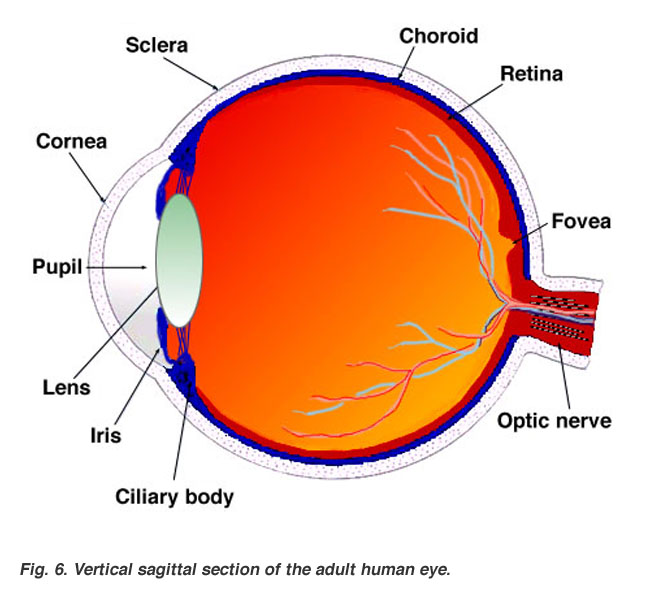
\includegraphics[width=0.5\textwidth]{simple-eye-anatomy}
    \caption{Simplified anatomy of the eye~\cite{webvision-images}.}
    \label{fig:vision:eye}
  \end{center}
\end{figure}

The retina is organized in layers of cell bodies or nerves,  Figure~\ref{fig:vision:simple-retina} shows a simplified version of the retina's anatomy~\cite{webvision-simple-retina}. Light enters the eye and has to travel all the way to the deepest part of the retina (right of Fig.~\ref{fig:vision:simple-retina}) to be sensed by the photoreceptors. 

\begin{figure}[h]
  \begin{center}
    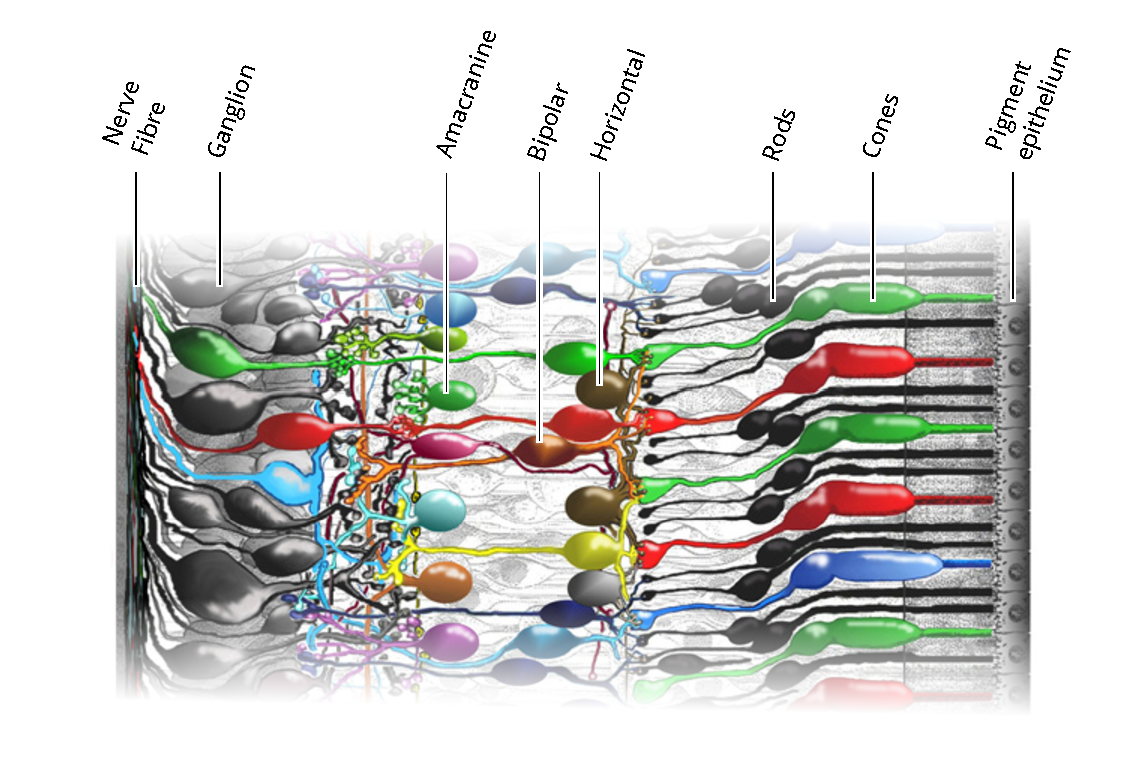
\includegraphics[width=0.7\textwidth]{retina-simple}
    \caption{Simple anatomy of the retina, adapted from~\cite{webvision-images}.}
    \label{fig:vision:simple-retina}
  \end{center}
\end{figure}

Photoreceptors transform light into an electrical signal. There are two primary types of photoreceptor cells within the retina: Colour is perceived by special type of receptors \emph{cones} and, contrast is perceived by \emph{rods}. Many mammals have retinas with more rods than cones, but primates' retinas are split in two separate zones. Most of the photosensitive area has more rods than cones but in a tiny region called the \emph{foveal pit}, there are almost no rods -- it's densely packed with cones. It is used for high-resolution vision and is virtually useless when there is not enough light~\cite{eye-brain-vision-hubel1995}.

The precise function of the other cell types is still a matter of debate and research. What is known is that \textbf{horizontal} cells  spatially average the input from photoreceptors and transmit to bipolar, which in turn output to ganglion cells. Horizontal cells also send a feedback signal to the photoreceptors, perhaps to adapt to different light conditions. \textbf{Bipolar} cells, as their name suggests, have outputs both to ganglion cells and photoreceptors. These first cell types (photoreceptors, horizontal and bipolar cells) use analog signals and feed ganglion cells which have a \emph{centre-surround} behaviour~\cite{eye-brain-vision-hubel1995,thompson2000brain}. Figure~\ref{fig:vision:centre-surround} illustrates the reaction of the two variants of centre-surround cells to different inputs.

\begin{figure}[h]
  \begin{center}
    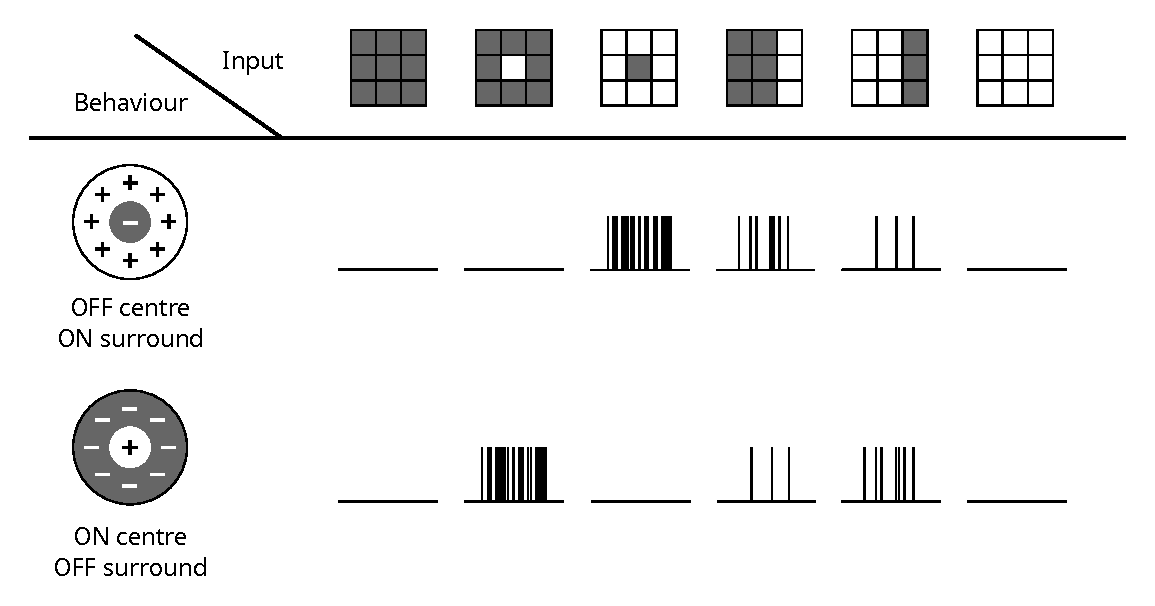
\includegraphics[width=0.7\textwidth]{centre-surround}
    \caption{Responses of centre-surround cells to different types of input.}
    \label{fig:vision:centre-surround}
  \end{center}
\end{figure}


\textbf{Ganglion} cells take input from bipolar cells, some form the surround (signal adapted by horizontal cells) and others the centre (pure signal from the photoreceptors). The centre-surround behaviour has been modelled by many authors using \emph{Laplacian of Gaussians} or \emph{Difference of Gaussians} ~\cite{thorpe-rate-coding-theory,virtual-retina,webvision-midget}. The output of ganglion cells are action potentials which are transmitted by the ganglion's axons, into the Lateral Geniculate Nucleus (LGN).

It's likely that most of the information sensed by the retina is redundant, this would keep the eyes working adequately even if some cells cease to function. To avoid saturation of nerve fibres and over-representation, lateral inhibition might play a big role~\cite{basab-model,thorpe-rate-coding-theory,field-sensory-coding}. The use of centre-surround responses in the retina is believed to help the eye overcome variations in lightning conditions, because the response comes from the contrast comparison between photoreceptors.

%After the light rays have been encoded into a neural representation, the optic nerve transfers the information to the Lateral Geniculate Nucleus (LGN) and from there to the visual portion of the cortex. A huge difference between a camera and the eye is that the latter maintains a continuous stream of information unlike the frame-based nature of cameras.